\subsection{Model Performance Comparison}
\begin{figure}[h]
    \centering
    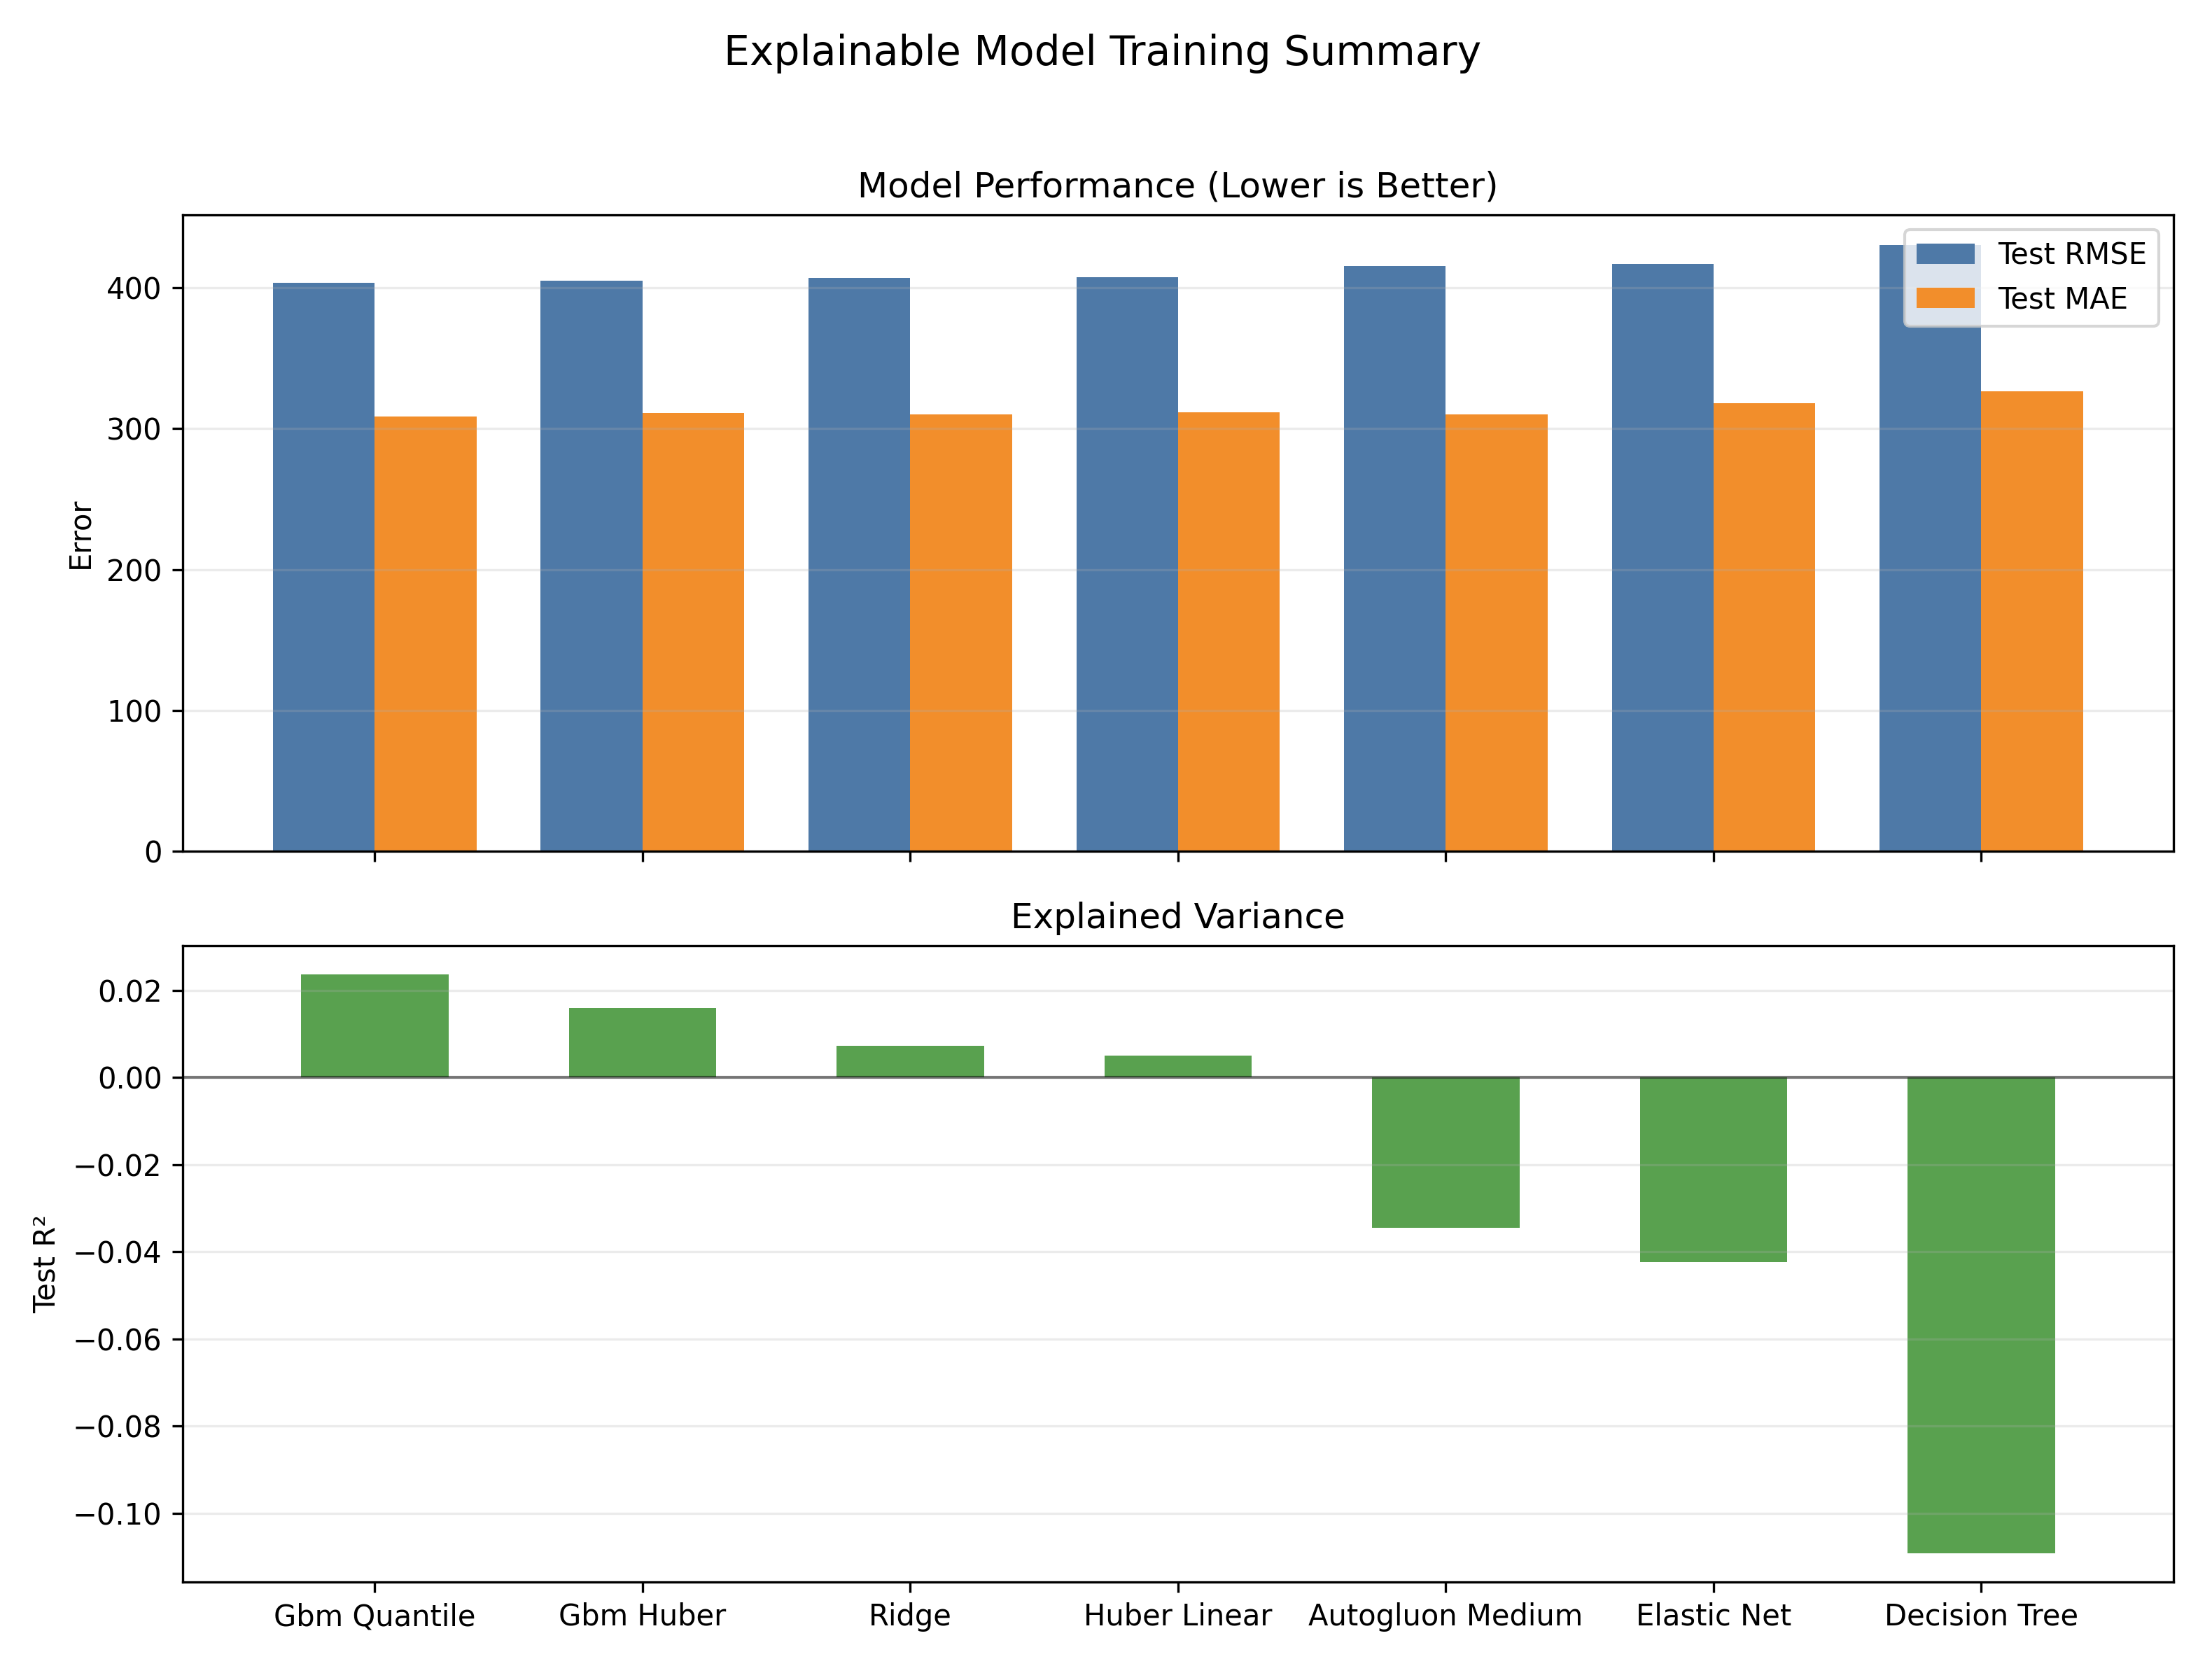
\includegraphics[width=0.92\linewidth]{../../../outputs/visualizations/model_performance.png}
    \caption{Test-set performance by model family (RMSE, MAE, and R\textsuperscript{2}).}
    \label{fig:model_performance}
\end{figure}

\textbf{What it shows:} Test RMSE and MAE are tightly clustered across models, and even the best R\textsuperscript{2} is near zero, so explained variance is limited.\\
\textbf{Why it is included:} It demonstrates that algorithm choice is not the current bottleneck; performance is broadly similar across model families.\\
\textbf{Recruiting implication:} Do not treat the model as a stand-alone ranking engine; use it as supporting evidence in a hybrid scouting workflow.

\subsection{Prediction Error Profile}
\begin{figure}[h]
    \centering
    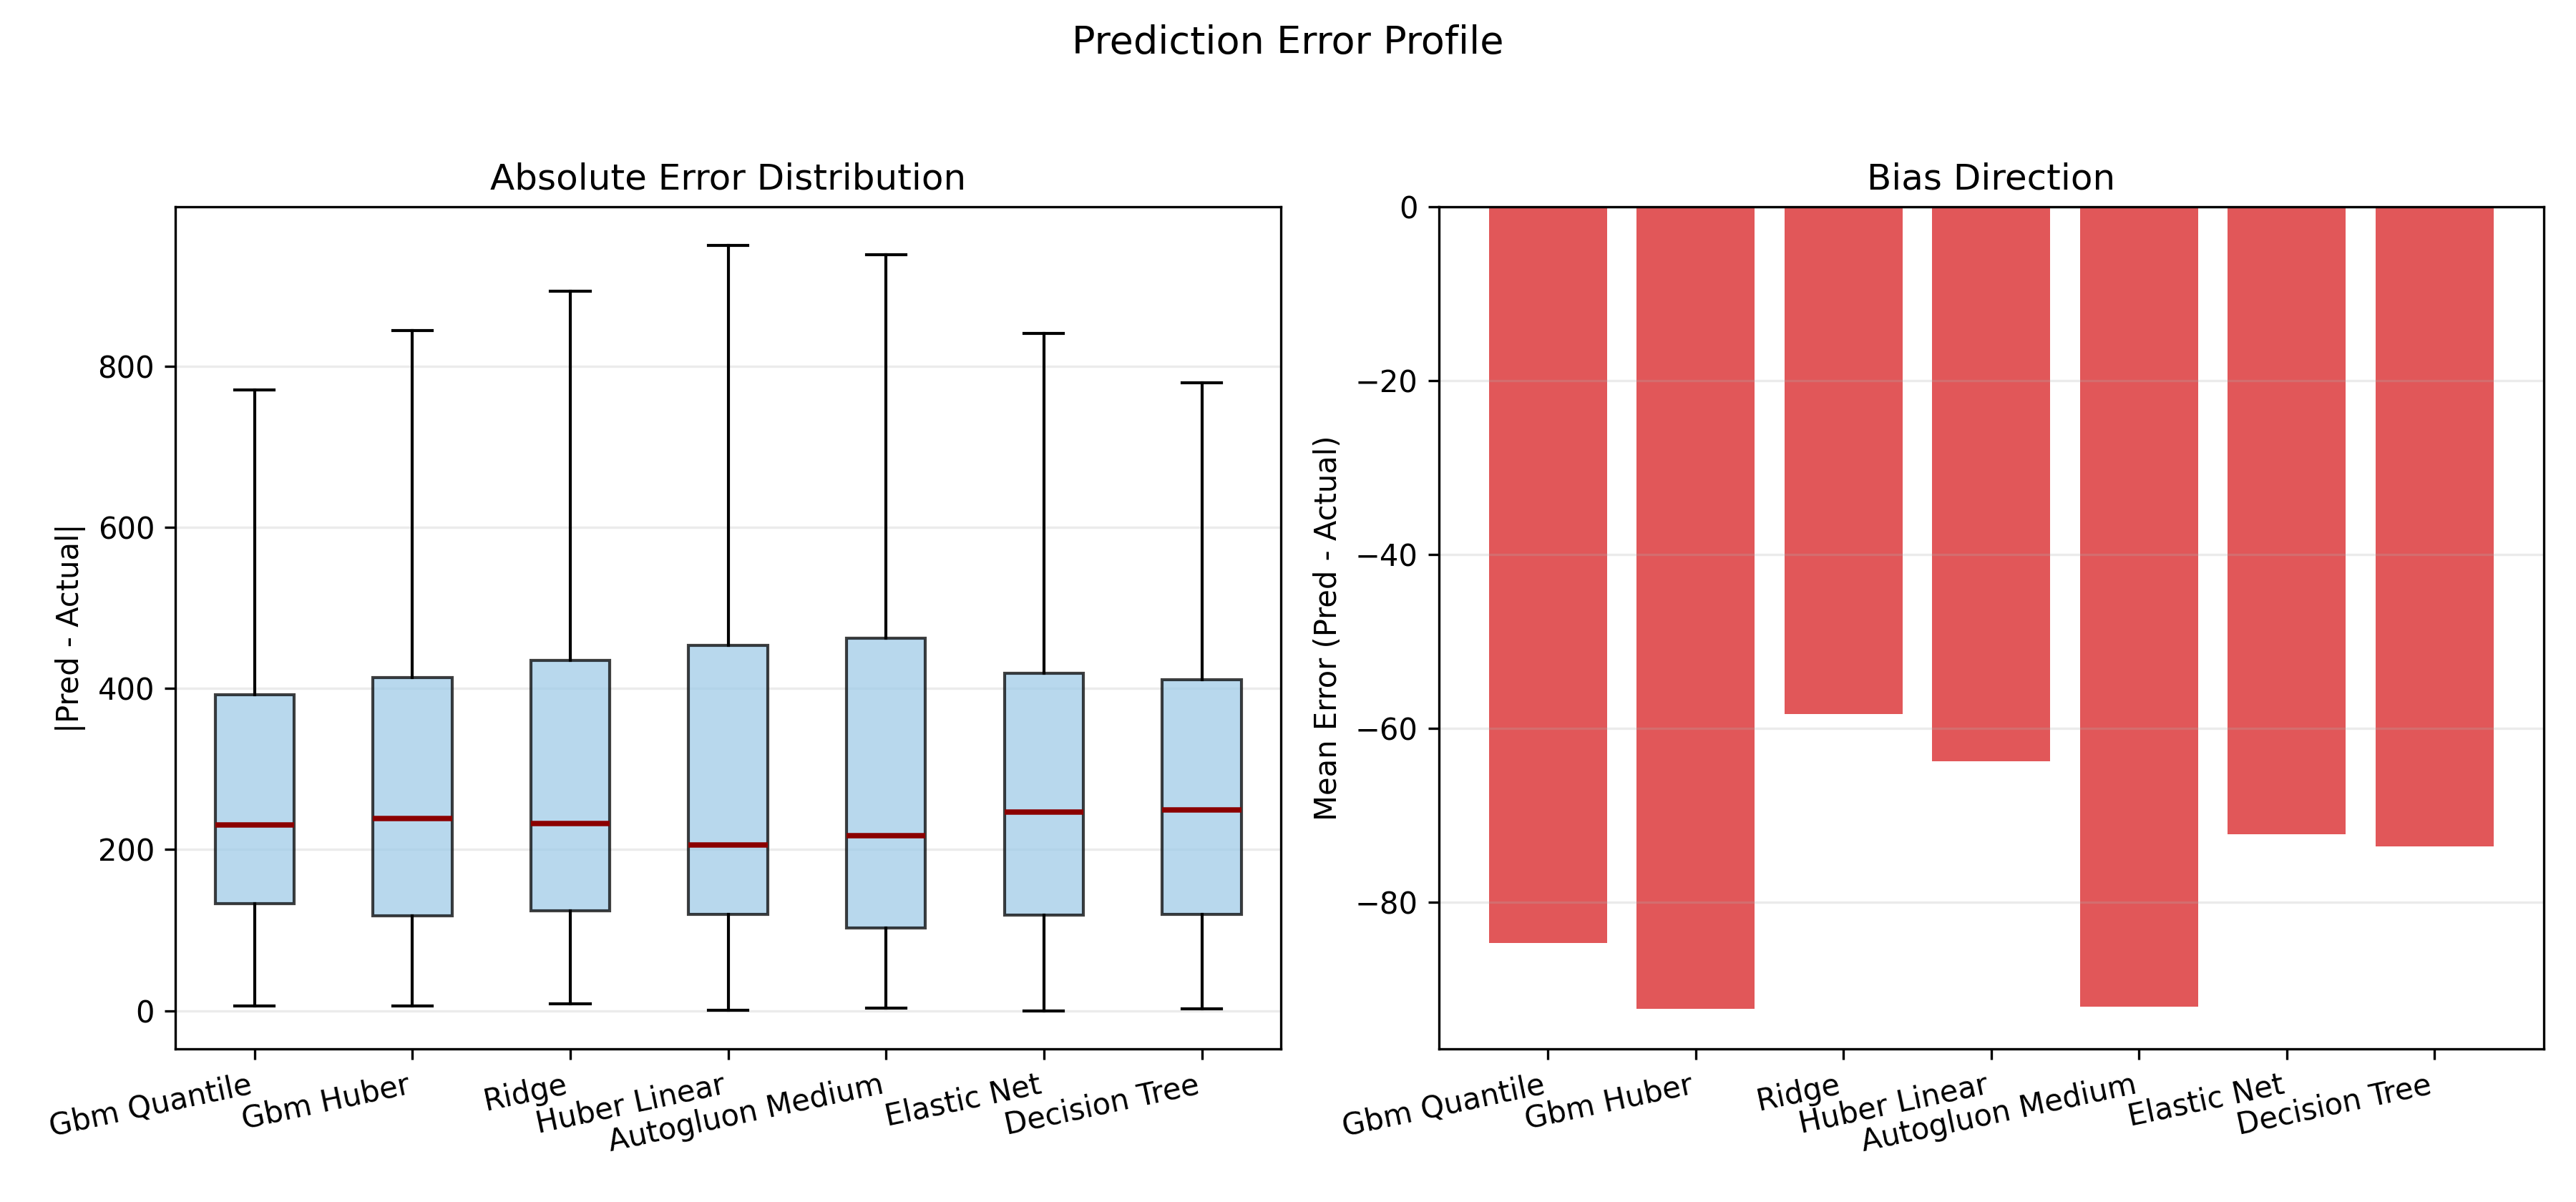
\includegraphics[width=0.92\linewidth]{../../../outputs/visualizations/prediction_error_profile.png}
    \caption{Error distribution, bias, and tail risk across candidate models.}
    \label{fig:prediction_error_profile}
\end{figure}

\textbf{What it shows:} All models have broad absolute-error distributions, negative bias (systematic underprediction), and large 90th-percentile errors.\\
\textbf{Why it is included:} It highlights reliability limits, especially in the high-upside tail where recruiting decisions are highest leverage.\\
\textbf{Recruiting implication:} Use outputs for coarse risk-tiering and flagging, not precise rank-order decisions on top prospects.

\subsection{Global Explanation Map}
\begin{figure}[h]
    \centering
    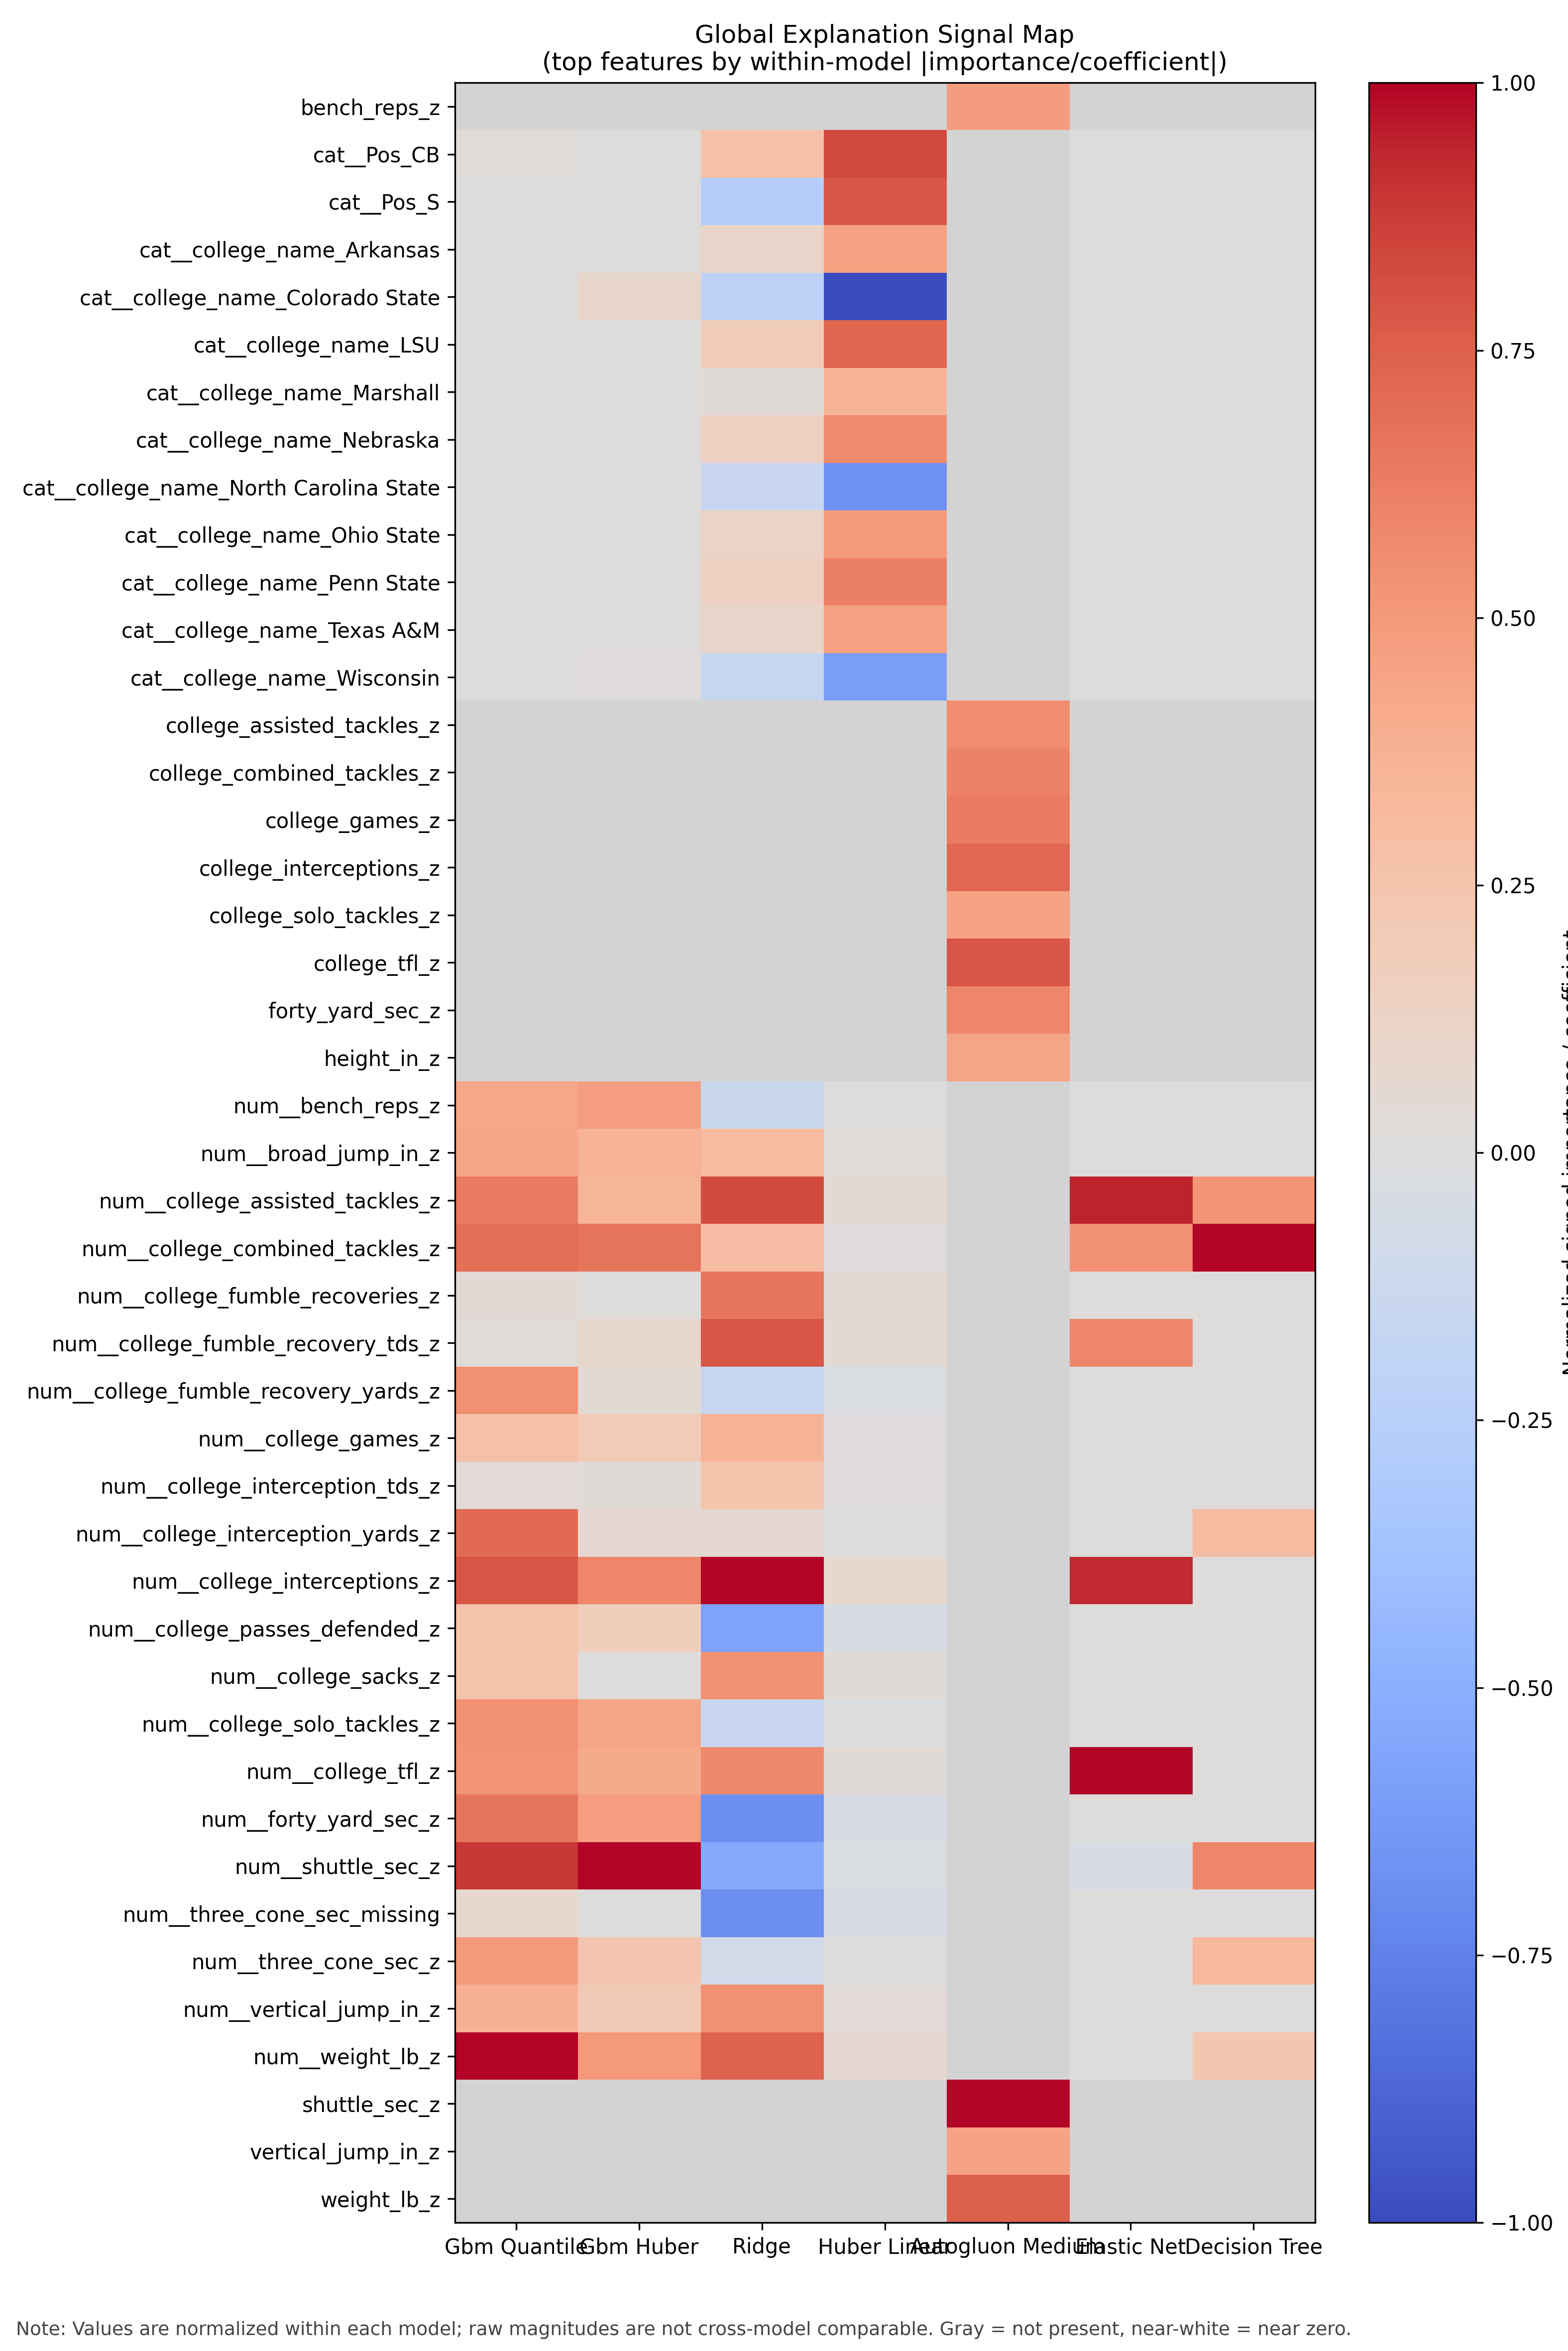
\includegraphics[width=0.92\linewidth]{../../../outputs/visualizations/global_explanation_map.png}
    \caption{Cross-model feature contribution map for directional signal discovery.}
    \label{fig:global_explanation_map}
\end{figure}

\textbf{What it shows:} Speed/agility measures (e.g., forty and shuttle), size, and selected college production metrics repeatedly appear among top-importance features.\\
\textbf{Why it is included:} Even with low overall accuracy, it surfaces stable directional signals that recur across models.\\
\textbf{Recruiting implication:} Prioritize these attributes in early screening, but treat them as guidance rather than a complete decision rule.

\subsection{NFL Production vs. Draft Round}
\begin{figure}[h]
    \centering
    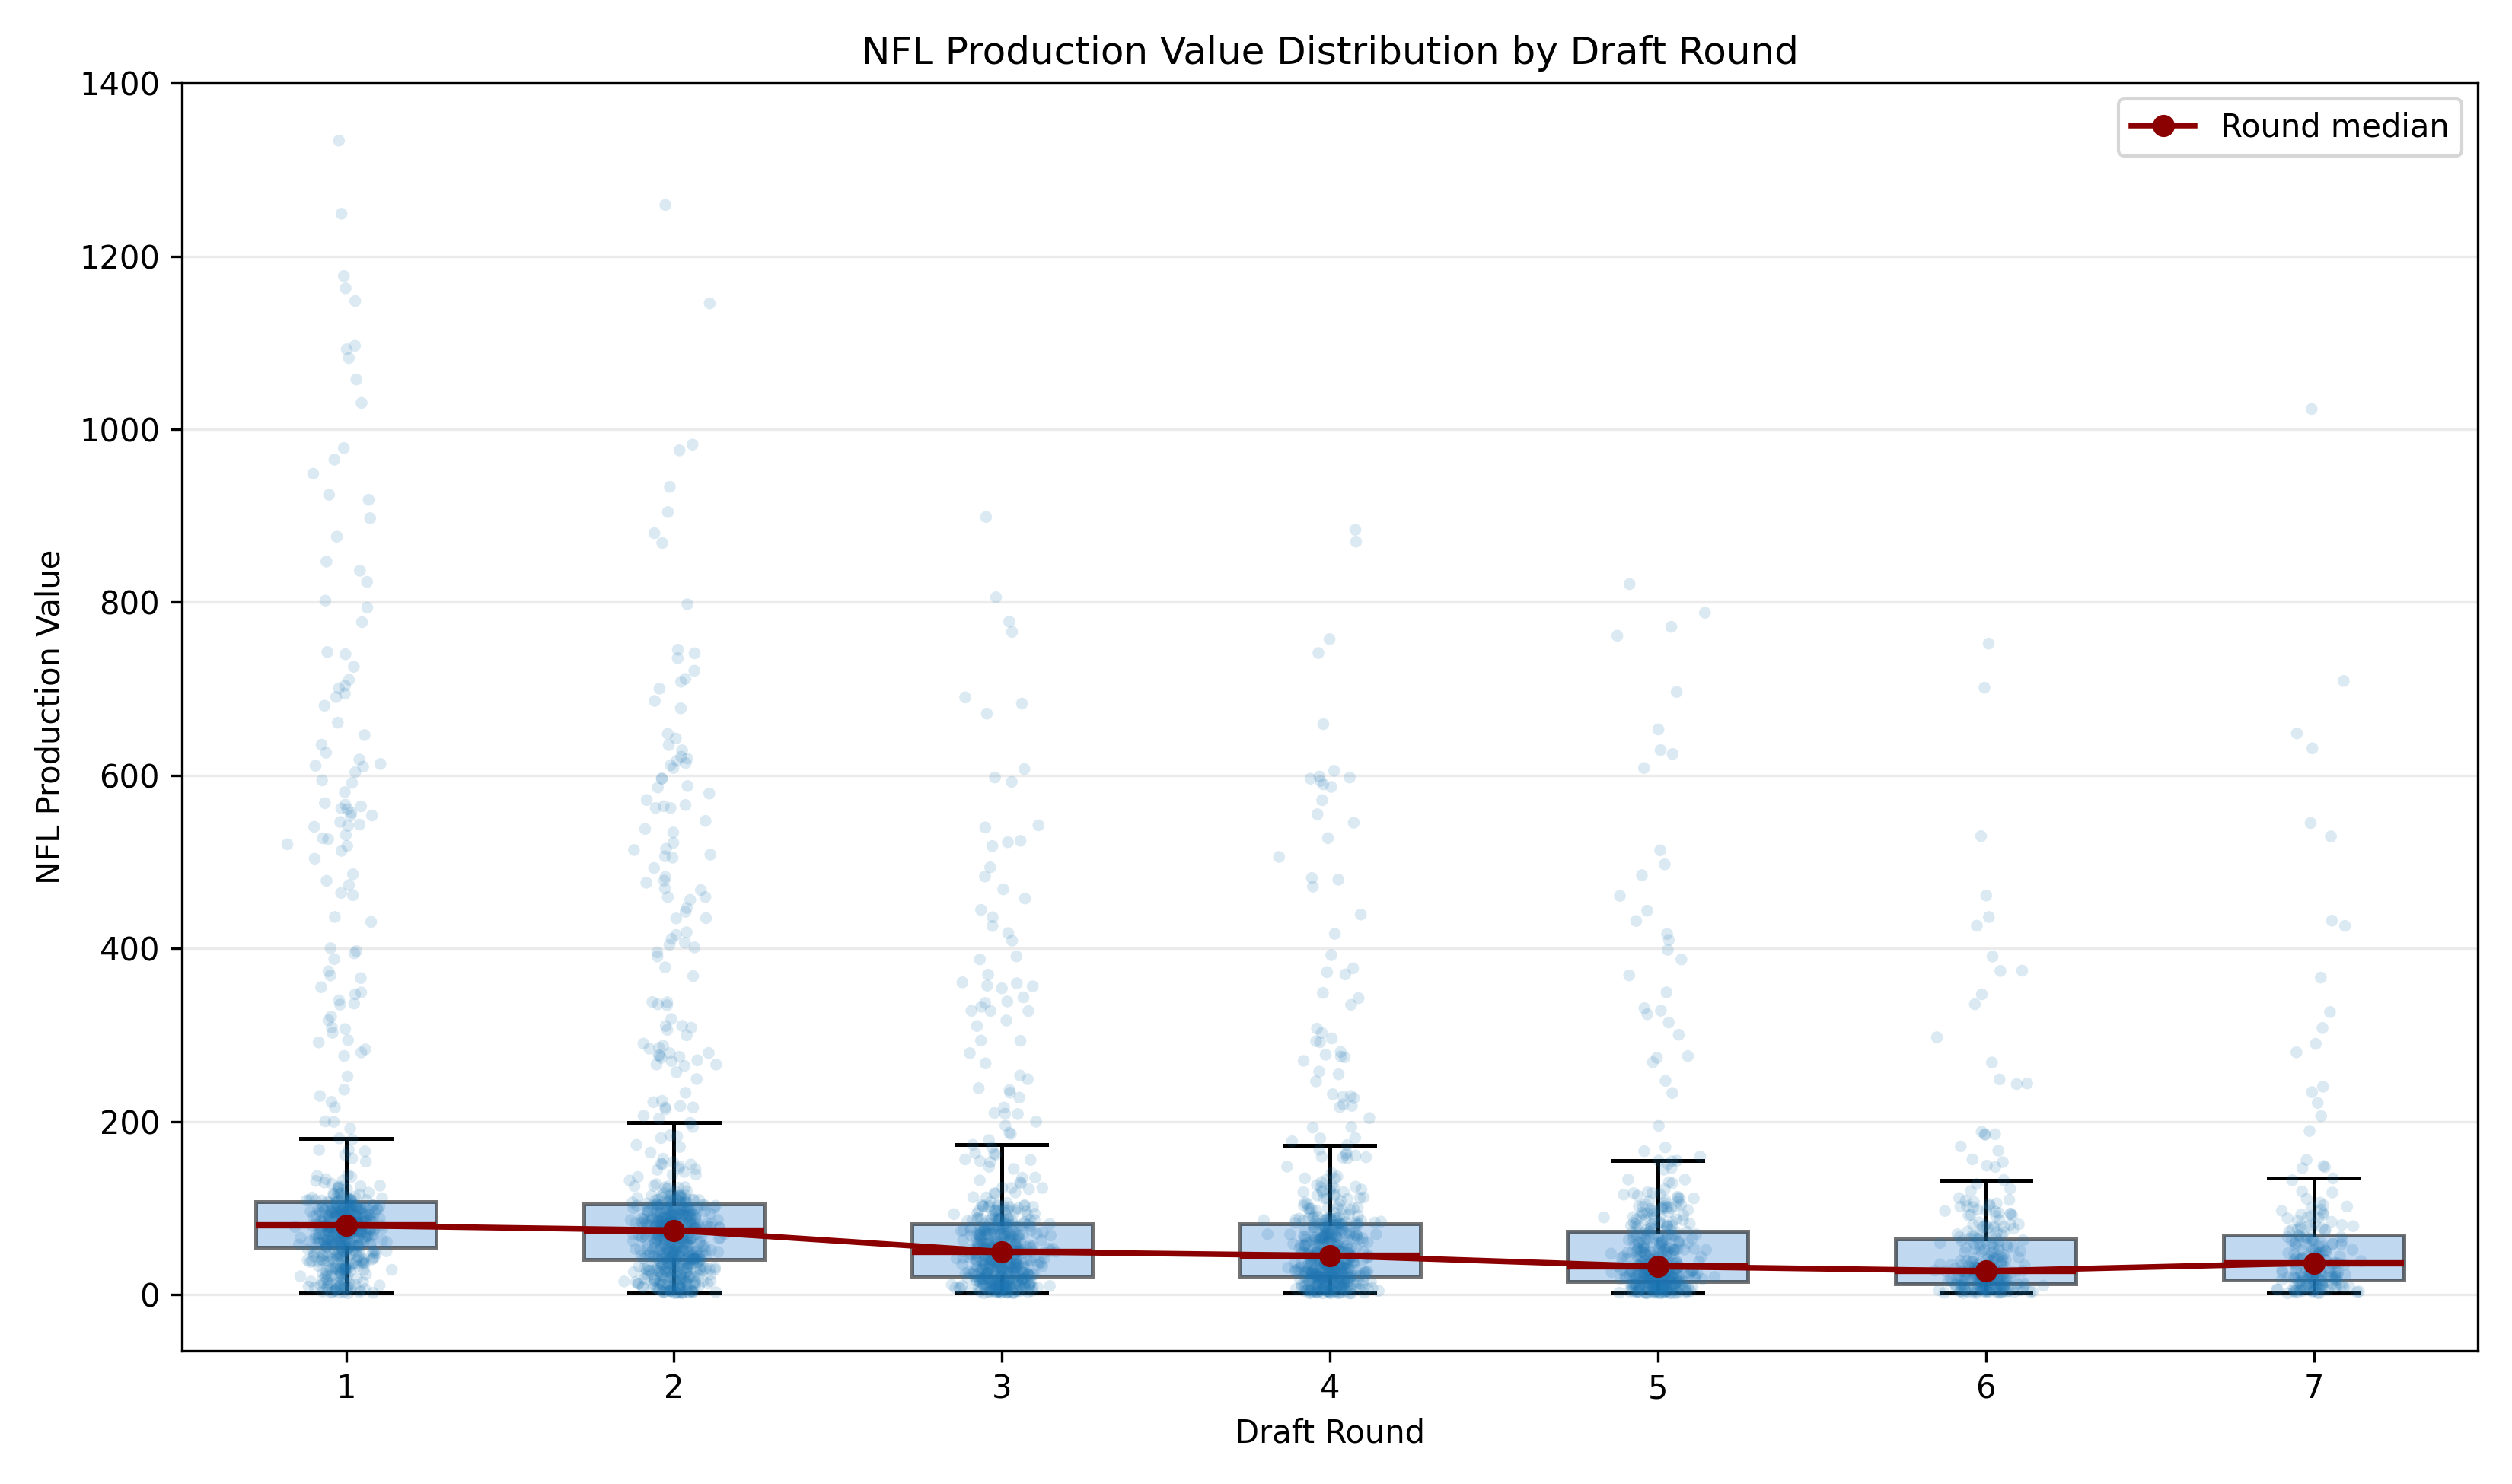
\includegraphics[width=0.92\linewidth]{../../../outputs/visualizations/nfl_production_vs_draft_round.png}
    \caption{NFL production distribution by draft round.}
    \label{fig:nfl_production_vs_draft_round}
\end{figure}

\textbf{What it shows:} Median NFL production generally declines in later rounds, but dispersion and overlap are substantial across all rounds.\\
\textbf{Why it is included:} It contextualizes baseline draft-capital signal while showing that late-round exceptions are common enough to matter.\\
\textbf{Recruiting implication:} Combine draft-round priors with context-rich college indicators to identify value outside early rounds.
